\section{Introduction}


Fourier series (FS) gives a new idea to expand a continuous and periodic signal with a series of trigonometric functions, which glanced at frequency analysis at the first time. Based on the idea of FS, other transformations were proposed to extend the limit on FS \cite{SignalSystem}: (1) Fourier transform (FT) for continuous but non-periodic signals; (2) discrete time Fourier transform (DTFT) for sampled signals; (3) discrete Fourier transform (DFT) for completely discrete analysis. These transformations make up Fourier transform family under Dirichlet conditions. Besides, Laplace transform extends the frequency into complex domain and Z transform simplifies DTFT practically.


Analysis in frequency domain provides more options to process signals or evaluate linear systems. For example, a spectrum given by fast Fourier transform (FFT, the fast algorithm for DFT) shows the frequency distribution of the signal; the location of poles and zeros of a system demonstrate the stability and dynamic properties.


In this paper, attentions are paid to digital signal processing. Power spectrum density is firstly introduced as a tool for frequency analysis and a new algorithm is delivered. Then the design and properties of some common used filters are discussed. Finally, an example is given to show processing procedure and the results.




\section{Power Spectrum Density}


DFT is used to analysis a certain signal. However, there are many kinds of stochastic signals whose statistical properties are the most concerned. As for a stationary and random signal, power spectrum density (PSD) is taken to estimate its properties in frequency domain \cite{SignalDetect}.


PSD is defined as the Fourier transform of the autocorrelation function of the given signal $x(t)$
\begin{equation}
    S_x(\omega) = \mathscr{F}\left(R_{xx}(\tau)\right) = \int_{-\infty}^{+\infty} R_{xx}(\tau) \iexp{-\mathrm{j} 2 \uppi \omega \tau} \diff \tau
\end{equation}
where the autocorrelation function $R_{xx}(\tau)$ is 
\begin{equation}
    R_{xx}(\tau) = \lim_{T\to \infty} \frac{1}{2T}\int_{-T}^{T} x(t) x(t-\tau)  \diff t
\end{equation}
Thus, the PSD is computed by
\begin{align}
    S_x(\omega) &= \int_{-\infty}^{+\infty} \left(\lim_{T\to \infty} \frac{1}{2T}\int_{-T}^{T} x(t) x(t-\tau)  \diff t t\right) \iexp{-\mathrm{j} 2 \uppi \omega} \diff \tau \notag \\ 
    &= \lim_{T\to \infty} \frac{1}{2T} \int_{-T}^{T} x(t)\iexp{-\mathrm{j} 2 \uppi \omega t} \left( \int_{-\infty}^{+\infty} x(t-\tau) \iexp{-\mathrm{j} 2 \uppi \omega \left(\tau-t\right)} \right) \diff t \notag \\
    &= \lim_{T\to \infty} \frac{1}{2T} \int_{-T}^{T} x(t)\iexp{-\mathrm{j} 2 \uppi \omega t} X^*(\jomega) \diff t \notag \\
    &= \lim_{T\to \infty} \frac{1}{2T} X(\jomega) X^*(\jomega) \notag \\
    &= \lim_{T\to \infty} \frac{1}{2T} \left| X(\jomega) \right|^2
        \label{eq:psd}
\end{align}
Eq~\eqref{eq:psd} is also known as Wiener–Khinchin theorem, which demonstrate the relationship between PSD and general frequency spectrum.




\subsection{Classical Power Spectrum Density Estimation}


Analog signals are analyzed based on the sampled data. Two important effects should be considered in sampling: (1) sampling should satisfy Nyquist sampling theorem, where the sampling frequency should be at least twice the maximum frequency of the origin signal. In practice, an analog anti-aliasing filter is usually used before the signal is sampled. (2) Finite sampling is equivalent to applying a window function to the infinite signal, which leads to frequency leakage effect. Because of these two effects, the PSD computed from the sampled data is just the estimation of the PSD of origin analog signal. That's why we usually say `spectrum estimation' instead of `spectrum calculation'.


The most direct method to estimate PSD is to discretize Eq~\eqref{eq:psd} using DFT and cancel the limit as below.
\begin{equation}
    S_x(\omega) \approx \frac{1}{T} \left| X(k) \right|^2 = \frac{1}{Nf_s} \left| X(k) \right|^2
\end{equation}
where $T$ is the total time of data, $N$ is the total number of points, $f_s$ is the sampling frequency. $X(k)$ is the DFT of $x(n)$, given by
\begin{equation}
    X(k) = \sum_{n=0}^{N-1} x(n) \iexp{-\mathrm{j} 2 \uppi \frac{n}{N}k} \label{eq:DFT}
\end{equation}
In the case where a window function $w(n)$ is applied to the sampled data, the PSD should be normalized as below. The $2$ in the numerator converts the two-sided PSD to one-sided PSD, whose square root is the most used in practice.
\begin{equation}
    S_x(\omega) = \frac{2}{\sum_{n=0}^{N-1} w^2(n) f_s} \left| X(k) \right|^2 \label{eq:periodogram}
\end{equation}


PSD can be estimated by combining Eq~\eqref{eq:DFT} and Eq~\eqref{eq:periodogram}. This direct method is called `periodogram'. Both MATLAB and Python provide built-in functions to calculate the periodogram. They are named \verb|periodogram| and \verb|scipy.signal.periodogram|. 


An example for PSD estimation is shown in Fig~\ref{fig:plotPSD}. The result of periodogram looks very noisy, especially in high frequency band. To improve the accuracy, Welch proposed a method by dividing the data into overlapped segments and computing the average of the periodogram of each segment.


\begin{figure}[!htb]
    \centering
    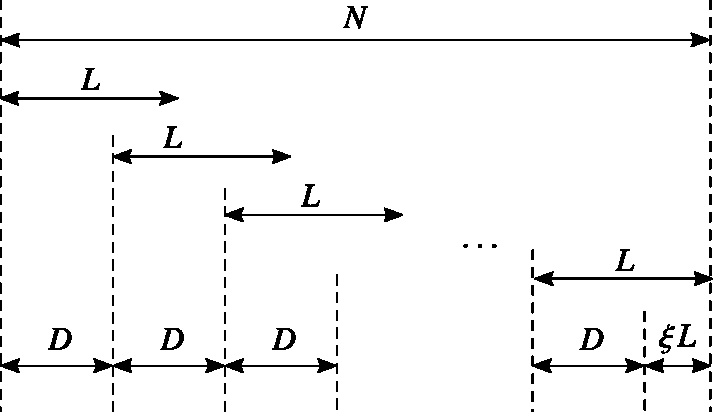
\includegraphics[width=0.5\textwidth]{Welch.pdf}
    \caption{The idea of Welch's method to estimate PSD.}
    \label{fig:Welch}
\end{figure}


The idea of Welch's method is shown in Fig~\ref{fig:Welch} and the relevant functions are \verb|pwelch| in MATLAB and \verb|scipy.signal.welch| in Python. 




\subsection{Logarithmic Frequency Axis Power Spectral Density}


As shown in Fig~\ref{fig:plotPSD}, by averaging PSD using Welch's method, the curve is less noisy. However, because the data is divided into segments, the length decreases, which decreases the frequency resolution. To further improve Welch's method, a new method named Logarithmic frequency axis Power Spectral Density (LPSD) was proposed \cite{LPSD}.


Considering that most signals occupy a wideband in frequency domain, the PSD is usually plotted with a logarithmic axis. Thus, the basic idea of the LPSD is to construct logarithmic frequency axis rather than linear axis. As a consequence, the frequency resolution changes with frequency, which allows dividing data into different segments. That is to say, the LPSD algorithm succeeds the idea of Welch's method and divides data according to the frequency point at which the PSD is estimated. The detailed procedure of the algorithm is discussed hereafter.


A logarithmic axis is made up of geometric progression, the length of which is assumed to be $J_{\rm des}$ and can be set manually, and it's not necessary equal to the length of data, $N$. The common ratio $q$ and ideal frequency resolution can be calculated as below.
\begin{gather}
    \lg f_{\rm max} - \lg f_{\rm min} = q\left(J_{\rm des} -1 \right) \quad \Rightarrow \quad q = \left(\frac{f_{\rm max}}{f_{\rm min}}\right)^{\frac{1}{J_{\rm des} -1}} = \left(\frac{N}{2}\right)^{\frac{1}{J_{\rm des} -1}} \\
    r_0(j) = f(j+1) - f(j) = \left(q-1\right) f(j)
    \label{eq:r0}
\end{gather}
Note that the maximum frequency is given by Nyquist frequency $f_{\rm max} = \frac{f_s}{2}$, and the minimum frequency is limited by the total sampling time $f_{\rm min} = \frac{1}{T} = \frac{f_s}{N}$. The index is denoted as $j$, which shows that the resolutions differ between frequencies.


However, the ideal frequency resolution $r_0(j)$ could be less than $f_{\rm min}$, which is not meaningful. So the resolution should be adjusted. To do so, we assume the desired number of segments to be $K_{\rm des}$, and the overlap ratio is $\xi$. So the desired resolution can be computed according to Fig~\ref{fig:Welch}.
\begin{gather}
    \left(K_{\rm des}-1\right) \left(1-\xi\right) L_{\rm des} + L_{\rm des} = N \\
    r_{\rm des} = \frac{f_s}{L_{\rm des}} = \frac{f_s}{N}\left(\left(K_{\rm des}-1\right) \left(1-\xi\right)+1\right)
\end{gather}
The ideal frequency resolution should be adjusted as below.
\begin{equation}
    r'(j) = \begin{cases}
        r_0(j) & r_0(j) \ge r_{\rm des} \\
        \sqrt{r_0(j)r_{\rm des}} & r_0(j) < r_{\rm des} \text{ and } \sqrt{r_0(j)r_{\rm des}} > f_{\rm min}  \\
        f_{\rm min} & \text{ else }
       \end{cases}  \label{eq:rp}
\end{equation}
Besides, the frequency resolution should consider an integer length of data and be further modified.
\begin{equation}
    L(j) = \left\lfloor \frac{f_s}{r'(j)} \right\rfloor \quad \Rightarrow \quad r(j) = \frac{f_s}{L_(j)} \label{eq:r}
\end{equation}
So far, the logarithmic frequencies can be computed by iterations given by Eq~\eqref{eq:r0}, Eq~\eqref{eq:rp} and Eq~\eqref{eq:r}. 


Similar to the Welch's method, $D$ and $L$ in Fig~\ref{fig:Welch} differ with index $j$. For $j$-th frequency point, 
\begin{equation}
    D(j) = \left\lfloor \left( 1-\xi \right) L(j) \right\rfloor
\end{equation}
and the number of segments is computed below.
\begin{equation}
    K(j) = \left\lfloor \frac{N-L(j)}{D(j)+1} \right\rfloor
\end{equation}


Average is usually deducted in PSD estimation. The average of $j$-th frequency point and $k$-th segment is given below.
\begin{equation}
    a(j,k) = \frac{1}{L(j)} \sum_{l=1}^{L(j)} x(D(j)(k-1)+l)
\end{equation}
Deducting the average and applying window function $w(j,l)$, the segment to be transformed is gained.
\begin{equation}
    G(j,k,l) = \big( x(D(j)(k-1)+l) - a(j,k) \big) w(j,l)
\end{equation}
The PSD of $k$-th segment at frequency $f(j)$ is calculated by single point DFT as below.
\begin{equation}
    A(j,k) = \sum_{l=1}^{L(j)} G(j,k,l) \iexp{-\mathrm{j} 2 \uppi \frac{m(j)}{L(j)} l}
\end{equation}
Note that the frequency index $m(j)=\frac{f(j)}{r(j)}$ is not necessary to be an integer.


Finally, the PSD at $j$-th frequency point is given by the average of $K(j)$ segments according to Wiener–Khinchin theorem.
\begin{equation}
    P(j) = \frac{C_{\rm PSD}(j)}{K(j)} \sum_{k=1}^{K(j)} \left| A(j,k) \right|^2
\end{equation}
The coefficient $C_{\rm PSD}(j)$ is used to normalize the PSD, which is given below.
\begin{equation}
    C_{\rm PSD}(j) = \frac{2}{f_s\sum_{l=1}^{L(j)} w^2(j,l)}
\end{equation}


The complete procedure of the LPSD algorithm has been discussed. The function is realized in both Python and MATLAB code, which can be found in the appendix. A comparison is given in Fig~\ref{fig:plotPSD}. The signal is obtained by filtering a white noise with elliptic filter so that the PSD should be equal to the gain of the transfer function theoretically.


\begin{figure}[!htb]
    \centering
    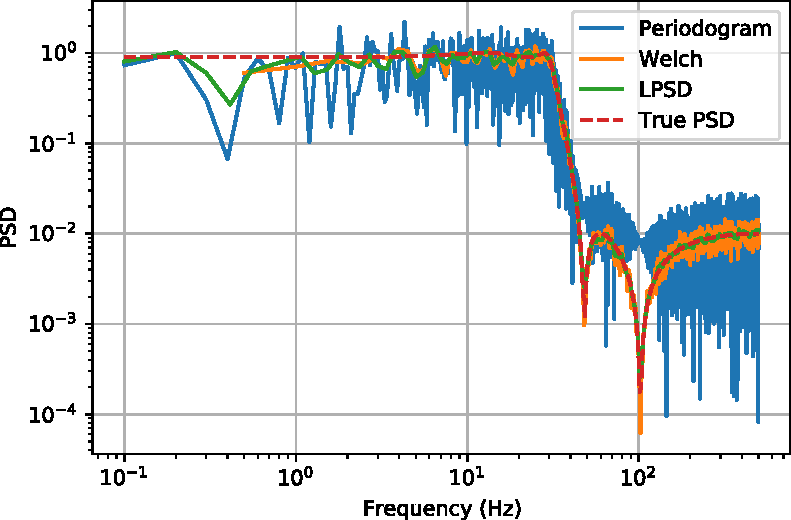
\includegraphics[width=0.6\textwidth]{plotPSD.pdf}
    \caption{Comparison of three methods to estimate PSD.}
    \label{fig:plotPSD}
\end{figure}


It's obvious that both the periodogram and the LPSD algorithms can calculate PSD at minimum frequency limited by the sampling time. But the result of periodogram is the most noisy. Welch's method improves the accuracy but sacrifices the minimum frequency. The LPSD provides the best estimated PSD, the result of which is very close to the theoretical value. However, the cost of the LPSD is to spend more time for calculation because it uses single point DFT and cannot benefit from FFT.




\section{Filter Design}


Properties of a given signal in frequency domain can be obtained from its PSD. To change these properties, a filter with certain frequency response should be applied to the signal. 




\subsection{Common Used Filters}


Since filter design has been a very proven technique, the theoretical analysis won't go far but some useful functions in MATLAB and Python will be introduced. Dynamic of an analog filter can be described in a differential function or a transfer function with Laplace transform as below.
\begin{gather}
    y^{(n)} + a_1 y^{(n-1)} + \cdots + a_n y = b_0 u^{(m)} + b_1 u^{(m-1)} + \cdots + b_m u \quad (m < n) \\
    H(s) = \frac{Y(s)}{U(s)} = \frac{b_0 s^{m} + b_1 s^{m-1} + \cdots + b_n}{s^{n} + a_1 s^{n-1} + \cdots + a_n} \quad (m < n)
\end{gather}
If there are poles in the transfer function, the filter would have infinite impulse response in time domain, for which we call it IIR filter for short.


To design a filter with built-in functions, properties of the filter shown in Fig~\ref{fig:filterdesign} should be specified. Taking low-pass filters as example, the frequency of passband is denoted by $f_{\rm pass}$ and $R_{\rm pass}$ is the allowed ripple. Stopband frequency is $f_{\rm stop}$ and the attenuation is $R_{\rm stop}$.


\begin{figure}[!htb]
    \centering
    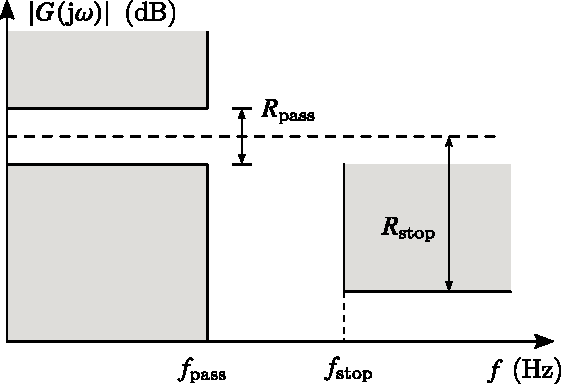
\includegraphics[width=0.5\textwidth]{FilterDesign.pdf}
    \caption{Filter properties specification.}
    \label{fig:filterdesign}
\end{figure}


Some common used filters are listed in Tab~\ref{tab:filterdesign} with MATLAB built-in functions for filter design \cite{matlabdoc}. In these functions, \verb|Wp| and \verb|Ws| are respectively the angular frequency of passband and stopband ($\omega_p = 2 \uppi f_{\rm pass}$ for example). Passband ripple \verb|Rp| and stopband attenuation \verb|Rs| are described in decibels. With the option \verb|'s'|, the function designs an analog filter. If a digital filter is desired, functions should be called without the option \verb|'s'| and \verb|Wp| and \verb|Ws| should be the digital frequency which is normalized by the sampling frequency.


For Python users, there are functions with the same names in \verb|scipy.signal| package \cite{scipydoc}. If the package is imported by \verb|import scipy.signal as signal|, a prefix \verb|signal.| should be attached to the functions to be called. Besides, the programming rules also has to be noticed. For example, the command \verb|[b,a]=butter(n,Wn,'s')| in MATLAB is equivalent to the command \verb|b,a=signal.butter(n,Wn,analog=True)| in Python.


\begin{table}[!htb]
    \centering
    \caption{MATLAB built-in functions for IIR filter design}
    \label{tab:filterdesign}
    \begin{tabular}{ll}
        \toprule
        Name & Built-in Functions  \\
        \midrule 
        Butterworth & \verb|[n,Wn] = buttord(Wp,Ws,Rp,Rs,'s');|        \\
                    & \verb|[b,a] = butter(n,Wn,'s');|                 \\
        Chebyshev Type I & \verb|[n,Wn] = cheb1ord(Wp,Ws,Rp,Rs,'s');|  \\
                    & \verb|[b,a] = cheby1(n,Rp,Wn,'s');|              \\
        Chebyshev Type II & \verb|[n,Wn] = cheb2ord(Wp,Ws,Rp,Rs,'s');| \\
                    & \verb|[b,a] = cheby2(n,Rs,Wn,'s');|              \\
        Elliptic Filter & \verb|[n,Wn] = ellipord(Wp,Ws,Rp,Rs,'s');|   \\
                    & \verb|[b,a] = ellip(n,Rp,Rs,Wn,'s');|            \\
        \bottomrule
    \end{tabular}
\end{table}


Comparison of four common used filters are shown in Fig~\ref{fig:filters} with options \verb|Wp=1|,\verb|Ws=3|, \verb|Rp=1|, \verb|Rp=40|. For the same target, elliptic filter has the least order but there are ripples in both passband and stopband. Butterworth filter has flat frequency response with passband, but the order is the largest, which means it takes more resources for calculation. Chebyshev filters have a compromise with order and ripple, where type I has ripples in passband and is flat in stopband, while type II is on the contrary.


\begin{figure}[!htb]
    \centering
    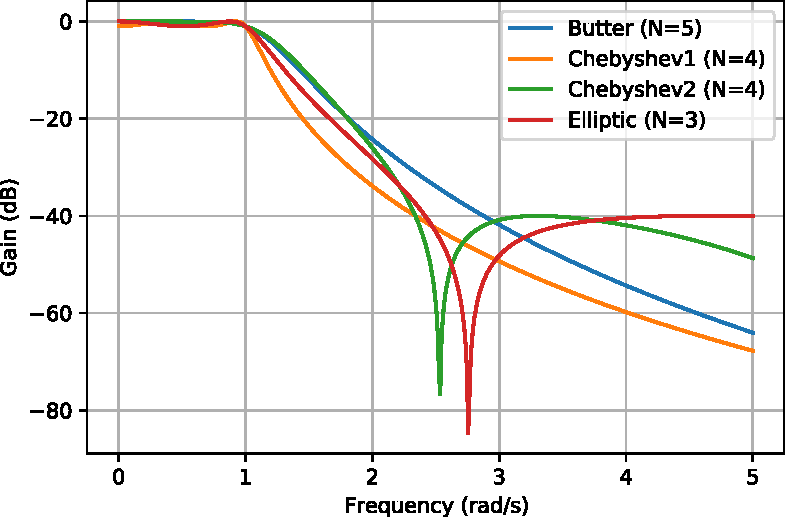
\includegraphics[width=0.6\textwidth]{filter.pdf}
    \caption{Comparison of four common used IIR filters.}
    \label{fig:filters}
\end{figure}


As has been mentioned, functions mentioned above can also be used to design digital filters. Besides, some methods such as `impulse invariance' and `bilinear' can be used to discretize an analog filter. Take an analog Butterworth low-pass filter for example, the discretized filter response is shown in Fig~\ref{fig:filter-c2d}. Note that the discretization could lead to aliasing effects, which may change the behaviors of the filter.


\begin{figure}[!htb]
    \centering
    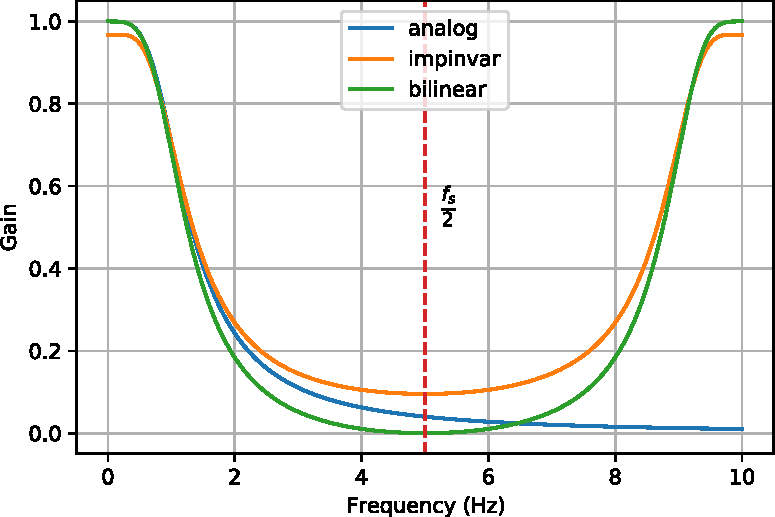
\includegraphics[width=0.6\textwidth]{filter-c2d.pdf}
    \caption{Digital filter design by discretization.}
    \label{fig:filter-c2d}
\end{figure}


Digital systems have a unique property which allows all-zero system to exist. These systems are described in difference equation or transfer function with Z transform as below.
\begin{gather}
    y(n) = b_0 u(n) + b_1 u(n-1) + \cdots + b_m u(n-m) 
     \sum_{k=0}^{m} b_k u(n-k) \\
    H(z) = \frac{Y(z)}{U(z)} = b_0 + b_1 z^{-1} + \cdots + b_m z^{-m} = \sum_{k=0}^{m} b_k z^{-m}
\end{gather}
The impulse response in time domain of this all-zero system is finite, thus this kind of filter is call FIR filter for short. Without poles, FIR filter is always stable.


Two methods are generally used to design a FIR filter. The first one is base on window function, whose idea is to apply a certain window function to the response of an IIR filter. MATLAB provides \verb|fir1| function to realize this design. For Python, the function is \verb|scipy.signal.firwin|.


Another method for FIR filter design is based on the frequency sample, where only filter order, frequencies and target responses are necessary. The function is named \verb|fir2| in MATLAB and \verb|scipy.signal.firwin2| in Python.


Applications with graphical user interface (GUI) are also available for filter design. They are \verb|filterBuilder| or \verb|filterDesigner| (or \verb|fdatool| in old version) in MATLAB and \verb|pyfdax| in Python \cite{pyfda}.


FIR filter is easy to realize in digital device while IIR filter has less order. Filter type should be selected according to the requirements and equipment constraints before it is designed. Design results should be checked, including stability, frequency response. Besides, for real-time applications, the filter must be causal.




\subsection{Zero-Phase Filtering}


The dynamic of the filter always leads to delay. To decrease the delay, an all-pass filter can be employed to adjust the phase response of the filter. As for sampled data, a technology name zero-phase filtering can be used. For digital filter with transfer function $H(z)$, there are four steps to realize zero-phase filtering \cite{mExamples}.
\begin{enumerate}[\indent Step (1)]
    \setlength{\itemsep}{0pt}
    \item Filter: $X(z) \rightarrow H(z)X(z)$ ;
    \item Reverse: $H(z)X(z) \rightarrow H(z^{-1})X(z^{-1})$ ;
    \item Filter: $H(z^{-1})X(z^{-1}) \rightarrow H(z)H(z^{-1})X(z^{-1})$ ;
    \item Reverse: $H(z)H(z^{-1})X(z^{-1}) \rightarrow H(z^{-1})H(z)X(z)$.
\end{enumerate}
The transfer function of the complete process $G(z)$ can be calculated as below.
\begin{equation}
    G(z) = H(z^{-1})H(z) = \left| H(\omega) \right| \iexp{\mathrm{j} \varphi (\omega)} \left| H(\omega) \right| \iexp{-\mathrm{j} \varphi (\omega)}  = \left| H(\omega) \right|^2
\end{equation}
There is no imaginary part in the transfer function so that no delay is introduced. From a practical point of view, when the data is reversed and filtered again, the same delay is introduced but in an opposite direction. Thus, the delay from the first filtering is compensated by the second filtering.


The function \verb|filter| in MATLAB or \verb|scipy.signal.lfilter| in Python can be used to filter data with specified filter. To apply zero-phase filtering, the function to be called is \verb|filtfilit| in MATLAB or \verb|scipy.signal.filtfilt| in Python. 


\begin{figure}[!htb]
    \centering
    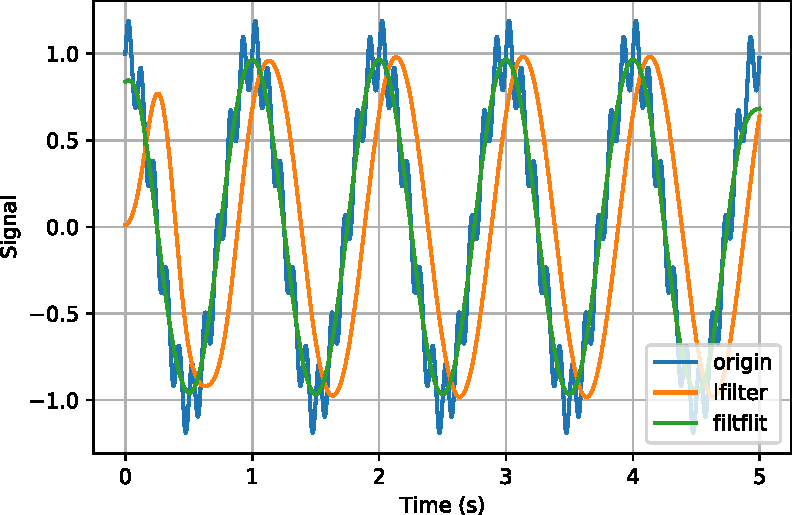
\includegraphics[width=0.6\textwidth]{ZeroPhaseFiltering.pdf}
    \caption{Comparison of normal filtering and zero-phase filtering.}
    \label{fig:zerofiltering}
\end{figure}


A comparison of normal filtering and zero-phase filtering is shown in Fig~\ref{fig:zerofiltering}. The delay of normal filtering is obvious. Attentions should also be paid to the transient performances. There is transient dynamic in the beginning due to the error of initial states. However, there is also transient dynamic in the end with zero-phase filtering, which is caused by the filtering of the reversed data at the third step. Unfortunately, zero-phase filtering is not causal, which means it cannot be used in real-time applications.





\section{Results}


Due to nonlinear properties, the AC current or voltage from the \SI{50}{Hz} power supply is polluted by some harmonic frequencies. To ensure the filter suppress the noise adequately, a simulation has been done whose input signal is listed in Tab~\ref{tab:input}.


\begin{table}[!htb]
    \centering
    \caption{Input signal for filter validation}
    \label{tab:input}
    \begin{tabular}{llllll}
        \toprule
        Frequency (\si{Hz}) & $50$ & $100$ & $150$ & $250$ & White Noise \\
        Amplitude (\si{A}) & $1.0$ & $0.3$ & $0.2$ & $0.1$ & $0.05$ (RMS) \\
        Phase (\si{deg}) & $0$ & $60$ & $-60$ & $-90$ & --- \\
        \bottomrule
    \end{tabular}
\end{table}


The length of data is $N=1000$ with sampling frequency $f_s=\SI{1}{kHz}$. The target is to filter out components with frequency above \SI{150}{Hz}. A Chebyshev Type II digital filter is chosen because IIR filter has less order and Chebyshev Type II provides flat frequency within passband. By Specifying $f_{\rm pass} = \SI{110}{Hz}$, $f_{\rm stop} = \SI{130}{Hz}$, $R_{\rm pass} = \SI{1}{dB}$ and $R_{\rm stop} = \SI{60}{dB}$, the designed filter is shown in Fig~\ref{fig:prjFilter}.


\begin{figure}[!htb]
    \centering
    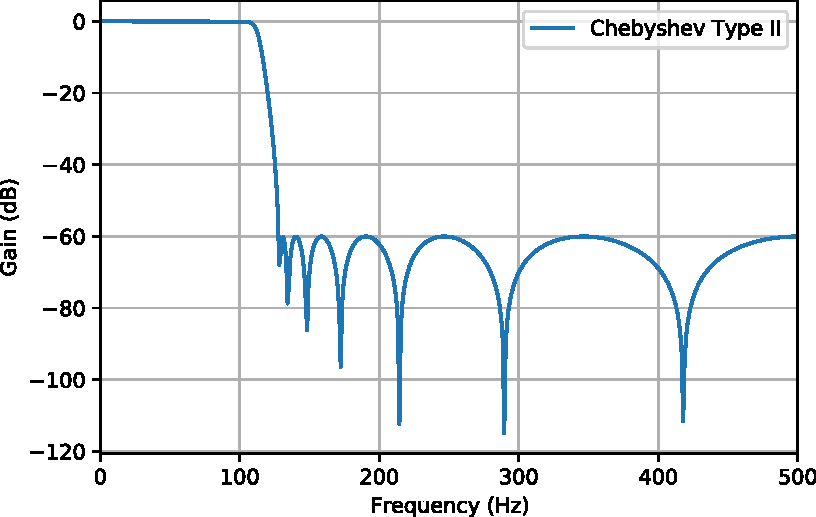
\includegraphics[width=0.6\textwidth]{prjFilter.pdf}
    \caption{Filter frequency response.}
    \label{fig:prjFilter}
\end{figure}


\begin{figure}[!htb]
    \centering
    \subcaptionbox{Signals in time domain.}{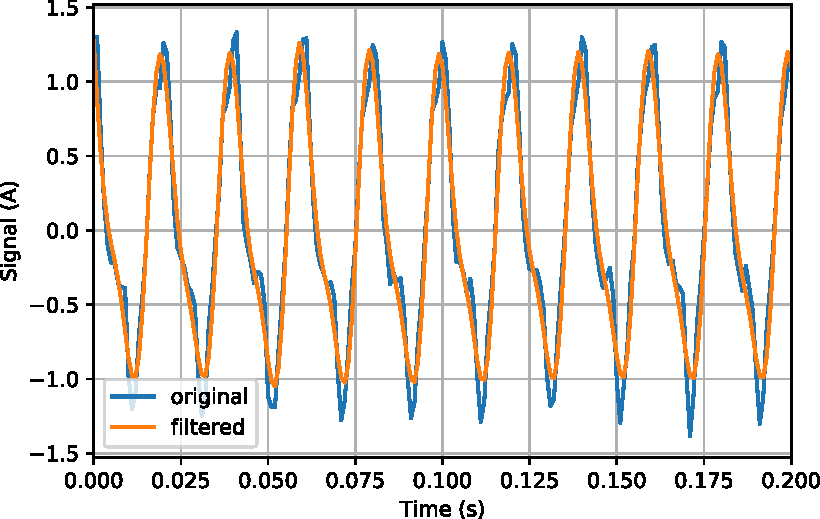
\includegraphics[height=4.9cm]{prjSignal.pdf}}
    \hfill
    \subcaptionbox{Signals in frequency domain.}{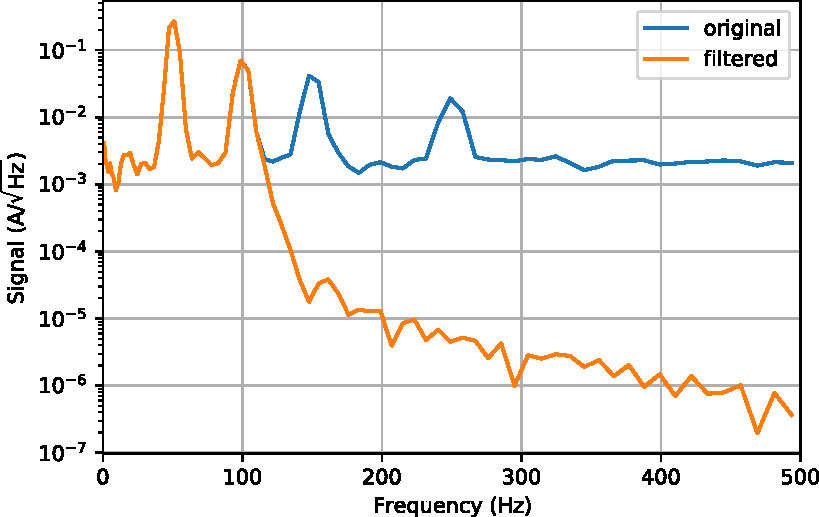
\includegraphics[height=4.9cm]{prjPSD.pdf}}
    \caption{Comparison of original and filtered signal.}
    \label{fig:prjSignals}
\end{figure}


Original signal is compared with filtered signal in Fig~\ref{fig:prjSignals} in both time and frequency domain. The zero-phase filtering technology was employed so that no delay is introduced. Because the high-frequency disturbances are removed, the filtered curve seems more smooth. For the PSD, it's obvious that the filter suppress high-frequency noise by about three orders of magnitude as stopband attenuation is set to \SI{60}{dB}.




\section{Conclusions}


In this paper, the LPSD algorithm is employed to estimate PSD, which takes advantage of minimum frequency range from the periodogram and succeeds the idea of averaging from Welch's method. Unable to embed FFT, the LPSD takes more time to calculate but provides more precise estimation with logarithmic frequency axis. Filters are designed with built-in functions and zero-phase filtering is used to filter data, which can compensate the delay caused by normal filtering. Zero-phase filtering is not causal, thus it cannot be used in real-time applications. A simulation was designed to validate the filter to suppress high-frequency disturbances from nonlinear effects of the \SI{50}{Hz} power supply. The results confirmed the properties of the filter and the PSD showed the disturbances in high-frequency band was suppressed by three orders of magnitude.